%%%%%%%%%%%%%%%%%%%%%%%%%%%%%%%%%%%%%%%%%%%%%%%%%%%%%%%%%%%%%%%%%%%%%%%%
%                                                                      %
%     File: Thesis_Results.tex                                         %
%     Tex Master: Thesis.tex                                           %
%                                                                      %
%     Author: Andre C. Marta                                           %
%     Last modified :  2 Jul 2015                                      %
%                                                                      %
%%%%%%%%%%%%%%%%%%%%%%%%%%%%%%%%%%%%%%%%%%%%%%%%%%%%%%%%%%%%%%%%%%%%%%%%
\chapter{Evaluation}
\label{chapter:results}

This chapter describes the evaluation of our V2X system, which comprises the PKI Manager and Vehicle Manager. The three main non-functional requirements of our V2X system are performance, security, and privacy. With this in mind, we intend to answer the following questions: 

\begin{enumerate}
	\item Since interoperability is a constant concern, does the system provide acceptable performance? 
	\item Does the system deliver the necessary conditions for vehicle privacy, authentication and overall security?
	\item Does the implemented V2X environment provide vehicle privacy at an acceptable cost?
\end{enumerate}


The following sections address these three questions, staring with the performance and resource usage tests, moving to the privacy and security concerns. 

%%%%%%%%%%%%%%%%%%%%%%%%%%%%%%%%%%%%%%%%%%%%%%%%%%%%%%%%%%%%%%%%%%%%%%%%
\section{Performance}
\label{section:performance}
Performance is a fundamental concern when testing systems that address a sensitive subject such as road safety. The most common metrics of performance are latency and throughput: latency is the time necessary to complete certain operations and throughput in our case is defined by the number of requests that the PKI Manager processes in a determined time frame. While latency gives us an idea on how fast users are able to use each service, throughput relates to the capacity of the PKI Manager to process multiple requests in a given amount of time.

Such two performance metrics correspond to the metrics measured by our tests to the PKI Manager at different variants. To perform this evaluation several tests were done regarding the backoffice application, and the interaction between the Vehicle Manager and PKI Manager. The environment in which they execute is the following: 

\begin{itemize}
	\item A single installation of the PKI Manager application as the server. 
	\item A basic but functional vehicular PKI including one Root CA, one Enrollment CA, and one Authorization CA.
	\item A single installation of the Vehicle Manager application as the client. 	
\end{itemize}
Our goal with this setup is to provide a simple but complete V2X environment, where we can use the installation of the PKI Manager to test the performance of the backoffice and RA Service, and use the Vehicle Manager to execute tests focused the resource usage of V2X communications. 

\subsection{PKI Manager}
The PKI Manager is the component of our system which comprises the web application. Therefore, the performance tests done to the PKI Manager have the main goal of understanding how the application behaves under different work load conditions. These tests focus on two aspects: latency measurements of the operations supported by the backoffice application, and the latency resulting from the communications between client vehicles and the PKI through the RA Service operations.

Because the PKI Manager tests involve client-server communication over the network, we executed them on two different machines connected through the same network. The server ran on an Asus laptop with 16GB of RAM and an i7 Intel CPU. For the backoffice testes, the URL was accessed on the browser of the second machine and the measurements were taken using the network tab on the browser's developers console. Regarding the tests to the RA Service, the client vehicles were generated on the second machine using \textit{Apache Jmeter} \cite{jmeter}, an open source software designed for testing the performance of web applications. This configuration allows us in both test suits to consider the latency introduced by the network communications and the latency of the processing time at the server. 


\subsubsection{Backoffice Application}
The operations performed by the administrator application are simple but essential in order to have a functional PKI to serve as the backbone of trust within V2X communications. The processing is mostly located at the V2X Library, creating a waiting period in the backoffice application. On the administrator side, it makes sense to only test the latency of the operations performed by one user only, as this application is not meant to be used by many users concurrently. Next, we take a look over the operations evaluated on the backoffice: the generation of keys and certificates. 

The operation to add a key involves the following steps: generating a cryptographic key using the V2X Library, then storing it on a keystore and its information on the database. The operation to add a certificate is more complex than the previous, as it also involves searching for the keys which will be relevant to issue the certificate. Because of this factor, we included on the add certificate test the number of keys that exist on the system to provide a comparing factor amongst the different latency times. For each operation the timer started when the form was submitted (POST) and stopped when the page finished loading (GET). The reasoning behind not considering the generation of CAs in the test suit comes from the fact that, unlike the tested operations, generating a CA consists only in creating a simple database object and storing it. 


In Table \ref{tab:table1} we can observe the time necessary to complete the operations involving our backoffice application, which preclude user interaction. Overall from the perspective of an administrator the results are reasonable and will not negatively affect the usability of the application. Regarding the operation to add a certificate, the operations for adding a single key or certificate are fast, taking on average 71.6 and 73.7 milliseconds. There is a linear relation between the time that the system takes to add a certificate and the number of keys that exist on storage. This happens due to the nature of the operation, in which the server has to query the database and the keystore in order to find the cryptographic keys of the subject and issuer before calling the V2X Library to issue the certificate, and finally storing it on the database. This increase in delay is not critical, as considering a realistic number of keys (i.e., in the order of a few dozen keys) it does not affect the user experience to a point that it is noticeable.

\begin{table}
	\renewcommand{\arraystretch}{1.2} % more space between rows
	\centering
	\begin{tabular}{lccc}
		\toprule
		Operation           & $Time$ & $Keys$& $StandardDeviation$ $$\\
		\midrule
		Add key          & 71.6ms & 1 & 14.0ms   \\
		Add certificate  & 73.7ms &4& 10.0ms     \\
		Add certificate  & 81.0ms &20& 13.5ms     \\
		Add certificate  & 103.0ms &30& 14.0ms     \\
		Add certificate  & 128.6ms &40& 16.0ms     \\
		Add certificate  & 178.7ms &60& 19.5ms \\
		\bottomrule
		\end{tabular}
		
		\caption{Time needed to add a certificate and a key, calculated over twenty measurements.}
		\label{tab:table1}
	\end{table}
	
	\subsubsection{RA Service}
	
	The RA Service API is the gateway from which the vehicles are able to interact with the PKI to request certificates. Comparing with the backoffice application, the operations done by the RA Service are more complex and subject to more load due to the possibility of concurrent requests from the client vehicles. Therefore, the tests done to this component are designed to evaluate the behaviour of the API at different levels of server load. Ideally, to ensure that the results are as close to the reality as possible, API load tests are run on a production or equivalent system. However, in our case this was not possible so the results may differ depending on the machine which they run. In the remaining part of this section we take a look at the performance tests performed to the RA Service starting with latency of the supported operations moving to the throughput measurements. 
	
	\paragraph{Latency}
	
	Figure \ref{fig:graphs2} shows the tests done to the RA Service: latency resulting from the configuration, enrollment and authorization of vehicles respectively. As discussed before, we used \textit{Jmeter} in order to test each end-point. This tool allowed us to configure different number of users or virtual threads and send concurrent requests to the server automatically. For each operation we performed a total of 50 tests across different thresholds of concurrent users. We started with one user, tested 10 times, then increasing the number of users in order to increase the load on the server and provide a comparing factor between the latency times. The plot for each operation relates the number of concurrent users to the time needed to perform the operation. The time is the average of 10 measurements, where each test was performed when the previous was done processing. For each test, \textit{Jmeter} started the timer when the POST request was submitted by the thread and stopped it once the response was received. Meaning that the processing time done at the client side to build the requests and verify the responses is not included in our test results. All three operations involve reading the database, and the V2X Library to decode the request and build a response. In addition to this, both the enrollment and authorization of vehicles use the library to validate the vehicle's request and issue the certificate. For the authorization end-point we tested both use cases, as represented by Figure \ref{fig:protocol_2}: the authorization process without the enrollment verification (c), and the full authorization process (d).
	
	\begin{figure}
		\begin{subfigmatrix}{2}
			\subfigure[Vehicle Configuration]{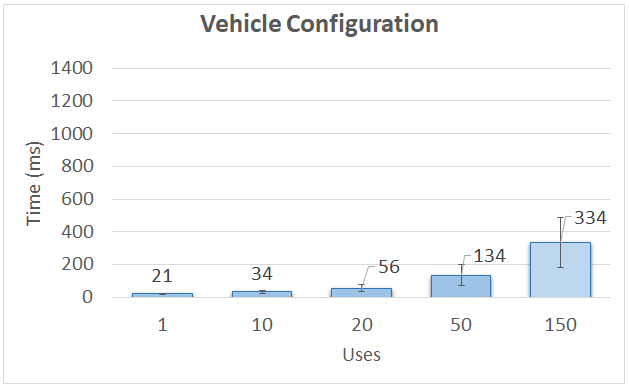
\includegraphics[width=0.49\linewidth]{Figures/conf_graph2.png}}
			\subfigure[Vehicle Enrollment]{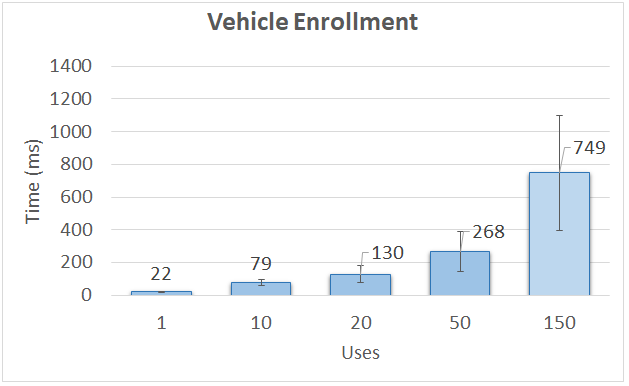
\includegraphics[width=0.49\linewidth]{Figures/enrol_graph2.png}}
			\subfigure[Vehicle Authorization w/o enrollment validation]{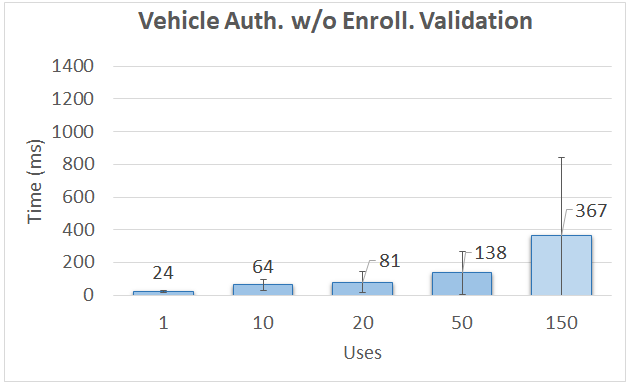
\includegraphics[width=0.49\linewidth]{Figures/new_auth_graph2.png}}
			\subfigure[Vehicle Authorization]{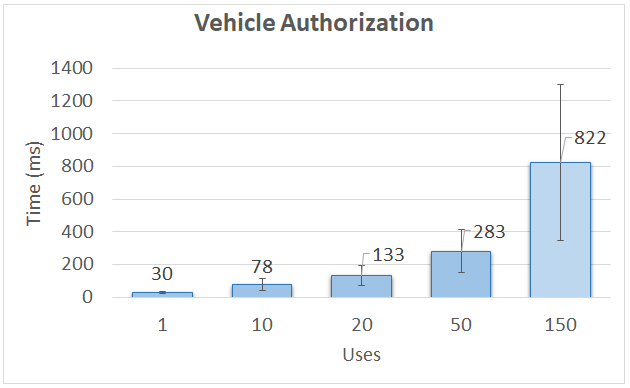
\includegraphics[width=0.49\linewidth]{Figures/auth_graph2.png}}
		\end{subfigmatrix}
		\caption{Latency measurements for the RA Service operations}
		\label{fig:graphs2}
	\end{figure}
	
	
	
	As we can see from the plot (d), the authorization of vehicles while verifying their enrollment is the operation which overall introduces more latency, with values varying from 30ms to 822ms. This happens due to the fact this operation is the most complex in terms of computation. Specifically, in the request validation where this version of the vehicle authorization requires the validation of two signatures: the signature that proves the possession of the verification keypair, and the vehicle's enrollment signature. In addition to this, the vehicle's enrollment credential is also verified.
	
	The second most expensive operation is the enrollment of vehicles (b) with latency values ranging between 22ms and 749ms. Comparing to the previous operation the enrollment of vehicles is simpler. The main difference comes from the validation of the vehicle's request, which in this case only requires the validation of two signatures: the canonical signature and the proof of possession signature. However, as we can see from plots (b) and (d) for all numbers of users the enrollment operation introduces almost as much latency as the more complex authorization, with values between 30ms and 822ms. This is because, unlike the previous operation, the enrollment of vehicles also requires saving on the database each enrollment credential issued, which introduces a bottleneck on the enrollment operation.
	
	Perhaps the most interesting comparison allowed by these tests is the comparison of the latency introduced by the two different vehicle authorization methods. As we can see from plots (c) and (d), the authorization without vehicle configuration introduced by our RA Service is on average faster than the standard full authorization flow. For example, considering the lowest server load of 1 user the new authorization flow represents an improvement of 16.6\% of the full authorization. As the number of concurrent users increases so does the improvement reaching its maximum value on the 150 user threshold with an improvement of 55.7\%. Since this version of the authorization is the most frequently used throughout the authorization process of the vehicles, the performance gains mean that the efforts presented in Section \ref{protocol} to optimize the authorization process as a whole were successful from a performance point of view. 
	
	The configuration of vehicles (a), being the simplest operation, introduced the least latency reaching a maximum of 334ms. Unlike the previous operations, the configuration of vehicles does not require signature validation at the application level or issuing certificates. It mainly requires decoding the request from the vehicle and read/writes to the database. However, the configuration of vehicles shares the same problem as the enrollment operation as the number of concurrent requests increases, i.e., database inserts become more and more expensive. At a 150 user mark it becomes almost as slow as the authorization of vehicles w/o enrollment validation (c), which is an operation that in terms of business logic is more complex. 
	
	One way to solve the problem shared by the configuration and enrollment operations is to increase the scalability of the data access layer by effectively managing the database writes. This can be achieved by using batch calls instead of single insert calls. Since we are using the default single insert calls, the number of writes results in same number of SQL \textit{insert} operations, which in turn result in that equal number of database round rips. Batching is a mechanism capable of grouping the \textit{inserts}, reducing the database round trips, and consequently increasing the performance of the data access layer. 
	
	\paragraph{Throughput}
	
	To test the throughput of the PKI Manager we used \textit{Jmeter} to generate requests to the vehicle authorization end-point since it is the most complex operation. This tool allowed us to configure five tests each with different ramp-up times. Each test was configured to 600 threads (users). The ramp-up period for each test was 60, 40, 30, 10 and 5 seconds respectively. Ramp-up period indicates the time duration that \textit{Jmeter} takes to start all the threads for that test. For example, if the ramp-up time is 10 seconds in a test with 10 threads it means that each thread will start after (10/10) 1 second. Having this mechanism in mind we reduced the ramp-up time in each test while maintaining the same number of users to increase of concurrency and work load on the server, providing a comparing factor between the resulting throughput measurements. It is important to note that, as explained in the documentation of \textit{Jmeter} \cite{throughput}, the throughput is calculated as (number of requests) / (total time) where time is calculated from the start of the first thread to the end of the last. For our tests the number of requests is constantly 600 and the total time is the period which took the test to fully execute. Specifically, starting with the first request (thread 1) and ending when the response to the last request is received (thread 600).
	
	Table \ref{tab:table2} relates the throughput measurements for each test done to the authorization of vehicles. In this table we can see the average latency of the 600 requests, the standard deviation of the latency, the throughput value, the percentage of failed requests and the test execution time. As we can see from the results, for the first three tests the server responded very well to the increase in the work load. We can see in the first test that for a ramp-up time of 60s the throughput was 10 requests per second. As the test was running for approximately 60 seconds, we can conclude that all the 600 requests were completed in approximately the same time as the ramp-up period meaning that the server was not delaying requests. This factor along with the low average request latency of 29ms, low standard deviation of 7.2ms and request error rate of 0\% allows us to conclude that this test was not able to reach the full capacity of the server. Therefore, the throughput was not higher because of the high ramp-up time that took to create the 600 requests. The same trend was maintained for two more tests, in the test with 30s ramp-up we can see that for twice the initial work load, the server responded with double throughput of 20 requests per second. This, along with the request latency still being low and no request errors is a further indicator the server was not yet saturated.
	
	However, once we increase the load by setting the ramp-up time to 10s the average latency of the requests started to increase to 592ms, which resulted in a higher standard deviation of 496.6ms as some requests were being processed fast while other were being delayed. For this test the throughput of the server was 52.8 request per second meaning that it was no longer increasing linearly in function to the increase in the work load. This is a sign that we are closer to reaching the server's capacity. Despite this, the average latency is still acceptable and because the error rate is 0 \% this test qualifies as a good performance output. As expected in the next test where we set the ramp-up to 5s, corresponding to twice the load as in the previous test, the throughput while still high (62.5/sec) increased at a lower rate comparing to the last 4 tests. The high average request latency of 2659ms and 12\% error rate on the requests is an indicator that we reached the full capacity of the server and for this work load it does not provide good performance.
	
	\begin{table}
		\renewcommand{\arraystretch}{1.2} % more space between rows
		\centering
		\begin{tabular}{lccccc}
			\toprule
			Ramp-up           & $Latency$& $Latency Standard Deviation$ & $throughput$& $TestTime$ $$\\
			\midrule
			60s          & 29ms & 7.2ms & 10.0/sec & ~60s  \\
			40s          & 28ms & 5.9ms & 14.9/sec & ~40s  \\
			30s          & 34ms & 5.6ms & 20.0/sec & ~30s \\
			10s          & 592ms & 496.6ms & 52.8/sec & ~11s \\
			5s           & 2659ms & 1480.6ms & 62.5/sec & ~9s \\
			\bottomrule
			\end{tabular}
			
			\caption{Throughput measurements to the authorize vehicle operation with 600 threads.}
			\label{tab:table2}
		\end{table}
		
		
		
		\subsection{Vehicle Manager}
		\label{section:memory}
		At the Vehicle Manager level, the focus of the latency/throughput metrics tests shifts from performance to resource usage. This is because the performance of the V2X communications could not be accurately measured by only using the Vehicle Manager. In the previous cases where the performance of the web application was tested we were able to relate the number of users to the latency needed to complete certain operations, which gave a general idea of how the system reacts under different work loads. This is not the case with the Vehicle Manager. The time needed to send messages from one vehicle to another (represented by objects within the Vehicle Manager) depends entirely on the system where the application is running. Without access to vehicle specialized V2X hardware the time taken by our testbed computer to generate, send and validate V2X messages is not conclusive. In addition to this, the network latency resulting from sending messages could not be accurately simulated because the communications within the Vehicle Manager's vehicles are represented by simple method calls. 
		
		In order to have a general notion of the possible quantities and the necessary storage capacity, Table \ref{tab:table3} lists the type of certificates, their size, and possible quantity. As described in Section \ref{etsi_design} all vehicles have to store different certificates on their local system. To estimate the size of the different certificates we used the \textit{java.lang.instrumentation} package \cite{instrumentation}, where we measured size of the ASN.1 COER encoded certificates (i.e. encoded using the V2X Library methods). Regarding the possible quantity of ATs stored within the vehicles, the values are estimated considering the AT usage pattern presented in Section \ref{section:at_usage}, assuming that a vehicle uses on average five certificates per day with a refill time of one year. In terms of numbers, the expected AT number can be calculated as (5 certificates) * (365 days) which equals to 1825 ATs. For the number of CA certificates we assumed a decently sized truststore installed on the vehicle. As we can see from Table \ref{tab:table3}, the authorization tickets and their corresponding private keys are the elements which demand more storage space (413.4KB), corresponding to approximately 87\% of total. It is also important to note that the number of the certificates can change from vehicle to vehicle depending on the usage pattern and the desired level of privacy, so the overall certificate storage demand may not be the same for different types of vehicles. This is further discussed in the following section.
		
		\begin{table}
			\renewcommand{\arraystretch}{1.2} % more space between rows
			\centering
			\begin{tabular}{lccc}
				\toprule
				Certificate & $Size$ & $Quantity$& $TotalSize$ \\
				\midrule
				Root CA         & 272 bytes & 20 &5.3KB \\
				Enrollment CA  & 288 bytes &100&28.1KB \\
				Authorization CA  & 288 bytes&100&28.1KB\\
				Enrollment Credential  & 208 bytes &1 & 0.2 KB\\
				Authorization Ticket  & 200 bytes &1825 & 356.4KB\\
				AT private key & 32 bytes & 1825 & 57.0KB\\
				\midrule
				\null  & \null & \null & 475.1KB\\
				\bottomrule
			\end{tabular}
			
			\caption{Estimated vehicle certificate storage demand}
			\label{tab:table3}
		\end{table} 
		
		\section{Security}
		\label{section:pricacy}
		In this section we analyse how our system achieves the security goals previously defined in Section \ref{goals}. In particular, we discuss the following security properties: confidentiality, data authenticity, and authorization.
		
		\subsection{Confidentiality}
		Confidentiality over the communications in an important characteristic of our system. Given that it falls outside the scope of V2X communications to restrict access to messages to certain users, the confidentiality aspect of our system only applies to the communication between the Vehicle Manager and PKI Manager.
		
		To ensure confidentiality, all the information transmitted from and to the client is sent through an SSL secure channel. In this communication channel the Vehicle Manager is authenticated, where the server requires its certificate in order to accept communications. 
		
		In addition, we also provide application level encryption where every certificate request is encrypted by the vehicle so that only the intended recipient CA is able to decrypt it. This feature combined with the encryption of the response to the original vehicle allows the confidentiality of the vehicle's identity, preventing its disclosure during the certificate requests.
		
		\subsection{Data Authenticity}
		Data authenticity enables the receiver of a message to confirm the origin and integrity of the data. In our system, this property applies to both the client-server communication and V2X messages.
		
		Regarding the Vehicle to PKI communication, the authenticity of the messages is achieved at two levels: first at the channel and then at the application levels. The sender of messages is the Vehicle Manager and the recipient is the PKI Manager. When the vehicles are manufactured, the RA trusts the new connections because of the SSL connection with the Vehicle Manager, which can be seen as the vehicle manufacturer. However, after the configuration of such vehicles the authenticity of their certificate requests is achieved at the application level, through the use of digital signatures.
		
		The authenticity of the V2X messages is a similar process where a vehicle being the recipient of a V2X message is able to trust the authenticity of the message by verifying the signature of the sender vehicle against a trusted certificate chain. 
		
		\subsection{Authorization and Authentication}
		Authorization over services requires user authentication. In our system this is applied in two aspects: the authentication of the administrator to manage the PKI and the client vehicles to request certificates. 
		
		The authentication of the administrator is accomplished through the use of a username/password mechanism, where the credentials are stored within the database of the server. Specifically, the password is hashed with the \textit{Bcrypt} algorithm before being saved to avoid mainlining it in clear text. The implementation of the hashing function is provided by \textit{Spring Security} and is prepared to internally generate and maintain a random salt value to be hashed alongside the password.
		
		The access to the data stored within the database is protected by username/password authentication. In addition to this, the access privileges are different depending on the type of user accessing it.
		
		Regarding the authorization of the vehicles, this is achieved through the RA service of vehicle configuration. Only vehicles which completed this service are recognized by our server and are able to request certificates.
		
		
		\section{Privacy}
		In our system preserving the privacy of users is one of the most important concerns. Losing privacy might mean that an attacker is able to track vehicles using the V2X communications, which is undesired. The main system variables that might affect the privacy of its users are the number of pseudonym certificates, and the usage pattern. The more pseudonym certificates a vehicle has available, the better is the privacy because the vehicle will have more choices when changing pseudonym. However, as described in the previous sections the increase of privacy comes with the overhead of the increase in certificate storage demand, number of individual certificate requests, and consequently processing at the vehicle. In this section we analyze different V2X scenarios, where we relate a vehicle's movement pattern, the pseudonym usage, possible types of attackers and the resulting level of privacy.
		
		\subsection{V2X Scenarios}		
		Regarding the types of vehicle trips, we wanted to choose real life cases where V2X communications could be involved. For the privacy scenarios we considered the following cases:
		\begin{itemize}
			\item \textbf{Vehicle A:} Round trip, the typical daily home to work commute.
			\item \textbf{Vehicle B:} One-way Trip, from point A to B.
		\end{itemize}
		
		
		The usage of certificates to sign V2X messages introduces privacy concerns over the communication. Therefore, the pattern which vehicles use pseudonyms and the frequency in which the certificate are changed are very impactful variables. We considered the following pattens:
		\begin{itemize}
			\item \textbf{Pattern A:} The vehicle always uses different pseudonyms.
			\item \textbf{Pattern B:} For a period of time the vehicle uses all the available pseudonyms then, if necessary, reuses the certificates in a different order.
		\end{itemize}
		
		To represent a challenge to the system's privacy, we choose different types of attackers differentiated by their power to capture messages within an area of operation.
		\begin{itemize}
			\item \textbf{Attacker A:} Controls a single section on the road while being able to visualize the victim vehicle and capture all messages.
			\item \textbf{Attacker B:} Controls two distant sections on the road where the victim vehicle will pass.
			\item \textbf{Attacker C:} Attacker is moving for a limited period following the victim vehicle. 
		\end{itemize}
		
		
		
		\subsection{Privacy Levels}
		
		Table \ref{tab:table3} organizes the scenarios from the lowest possible privacy to the highest.
		
		\begin{table}
			\renewcommand{\arraystretch}{1.2} % more space between rows
			\centering
			\begin{tabular}{lccc}
				\toprule
				Vehicle Type           & $CertificatePattern$& $VulnerableToAttacker$ &$PrivacyLevel$ $$\\
				\midrule
				A      & B      & A,B,C & Low\\
				B      & B      & B,C & Medium\\
				A      & A      & C & High\\
				B      & A      & C & High \\
				\bottomrule
				\end{tabular}
				
				\caption{Privacy scenarios ordered by level of privacy.}
				\label{tab:table3}
			\end{table}
			
			\subsubsection{Low Privacy}		
			Starting with the least privacy, vehicles of type A (round trips), using and reusing certificates as in th pattern B with low pseudonym change (e.g. using the same certificate for hours) are vulnerable to all types of attackers. Considering the attacker A there is a window of vulnerability if the vehicle passes the area controlled by the attacker twice with the same pseudonym. In this case the attacker is able to map that pseudonym to the victim's vehicle. Eventually, when the vehicle reuses the compromised pseudonym it may be possible for the attacker, if capturing the messages, to infer the vehicle's route. The same situation happens when considering the attacker B but with a bigger window of opportunity as the vehicle passes the areas controlled by the attacker twice as more. Because the frequency of certificate change is low it directly affects the privacy of the vehicle when considering the attacker C. In this case, the longer the vehicle uses the same certificate the bigger the probability of the attacker seeing that constant message broadcast by the vehicle, therefore mapping the used pseudonym to the identity of the vehicle and enabling short-term tracking. Despite the fact that this pseudonym usage pattern is worst in terms of privacy for the vehicles usually commuting, it is the least expensive in terms of certificate storage demand because the vehicle is reusing certificates with a low change frequency. 
			
			A privacy improvement for the same conditions (Vehicle type A, and certificate pattern B) would be to increase the frequency in which the vehicle changes pseudonyms. In this case, the vehicle would be more protected against the three types of attackers. In the case of attacker A and B, this is achieved because it would reduce the risk of the vehicle still be using the same certificate while passing through the zone(s) controlled by the attacker. The increase in privacy against attacker C is based on the unlinkability attribute of the pseudonym certificates. This means that when a vehicle changes pseudonym the new certificate can not be mapped to the old, therefore reducing the ability of the attacker to infer which certificate belongs to the vehicle. However, in order to assure the unlinkability of the pseudonym certificates care must be taken regarding the aggregation of information written on the certificate. For example, if a set of the vehicle's certificates have the exact same expiration date an attacker could infer that they belong to the same vehicle, disrupting the unlikability of the affected certificates. 
			
			\subsubsection{Medium Privacy}
			Medium privacy is achieved for vehicles of type B (one-way trips) using the certificate pattern B. In this case the vehicle can expect an improvement in the privacy level because it does not pass the same road twice. This is particularly effective when considering attackers of type A and B which control fixed areas of such road. For the first type of attacker, it is only possible to map a certificate to the vehicle if the vehicle passes the controlled area twice on different trips using the same certificate. Regarding the attacker B, it is possible to compromise a certificate if the vehicles passes the two controlled areas using the same certificate. As in the previous case, increasing the certificate change frequency will further decrease the power of the three attacker to compromise certificates for when the vehicle reuses them.
			
			
			\subsubsection{High Privacy}
			The best privacy for all vehicle types is achieved through the usage the certificate pattern A. Because certificates are not reused, even if the attacker manages to map a pseudonym to the victim's vehicle it is only possible to track the vehicle for the duration that it uses that certificate (short-term tracking). Increasing the certificate change frequency will further reduce the power of the attacker. 
			
			
			
			\subsection{Discussion}
			A general rule of thumb that is important to consider when using pseudonyms is that a pseudonym is only effective in a crowd. In vehicular communications this means that a pseudonym certificate is only effective if there are more vehicles around using them. If a vehicle is isolated on a road sending V2X messages signed with a pseudonym certificate then that certificate can be immediately mapped to the sender, even considering a high pseudonym change frequency.
			
			We have seen in the scenarios presented above that pseudonyms are particularly vulnerable to reuse attacks where the attacker is able to map a specific certificate to a vehicle. In this case the pseudonym becomes compromised because the attacker will be able to link that certificate to the vehicle when it reuses it. The more certificates are compromised the bigger the chance of the attacker to infer a vehicle's route by observing the compromised certificates being reused at different locations. However, assuming that vehicles carry thousands of pseudonyms, a few compromised certificates might not be conclusive for the attacker. It all depends on the power of the attacker to compromise certificates by controlling areas and/or following the victim vehicle, the number of certificates reused by the vehicle, and the randomness in which they are selected. 
			
			We also have seen that having a low pseudonym change frequency is particularly vulnerable to short-term tracking attacks where the attacker is following the vehicle and is able to: (a) see the vehicle using the certificate while isolated, or (b) infer it by the captured messages which are signed constantly by the same certificate. We concluded that the best way to preserve privacy is to increase the number of pseudonyms, which enables the possibility of a higher pseudonym change frequency and lowers the need to reuse certificates. 
			
			More concretely, the price in terms of storage in order to have acceptable privacy depends on the travel distance of the vehicles. In the previous section, we estimated that if a vehicle uses on average 5 pseudonyms in a day with a refill time of one year it would need approximately 486.6KB of certificate storage space. Depending on the distance that a vehicle travels each day, it may need to use more that 5 certificates resulting in the reusage of certificates, and privacy loss in most cases. To assure that this does not happen a vehicle that spends more time on the road needs more certificates. For example, assuming a vehicle changes certificate each 10 minutes and an average travel time of 2 hours each day. The vehicle would need approximately 12 certificates a day in a total of 4380 for a year. Assuming the same number of PKI certificates as in the previous section \ref{section:memory}, this number of pseudonyms would increase the storage demand to approximately 1MB.
			
			
			\section{Sumary}
			In this chapter we presented the evaluation results of the developed V2X system. We started by evaluating the performance of the PKI Manager, then looked at the resource usage of the Vehicle Manager and finished by discussing the security properties and privacy of the system.
			
			The performance of the PKI Manager was measured at two different variants: the backoffice application and the RA Service. In the evaluation of the backoffice we measured the latency of the most complex PKI operations, the generation of keys and CA certificates. We concluded from the results that the measurements were reasonable, considering the complexity of the operations, and would not negatively affect the usability of the application by an administrator. From the results it was possible to conclude that the most expensive operations in terms of latency are the full authorization and enrollment of vehicles. The new authorization of vehicles introduced by our RA Service was faster than the standard full process. 
			
			Lastly we presented how our system provides the security properties of confidentiality, data authenticity and authorization in both vehicle to PKI and V2X Communications. We concluded this chapter by analyzing how the privacy of the vehicles is maintained in V2X communications, discussing the different levels of privacy achieved by different vehicle types and pseudonym usage patterns.
			
			%%%%%%%%%%%%%%%%%%%%%%%%%%%%%%%%%%%%%%%%%%%%%%%%%%%%%%%%%%%%%%%%%%%%%%%%
